\documentclass[
oneside
]{scrreprt}
\usepackage{amsmath}
\usepackage{amsfonts}
\usepackage{amsxtra}
\usepackage{fontspec}
%\usepackage[default]{sourcesanspro}
\usepackage{xcolor}
\usepackage{amssymb}
\usepackage[backref=false,
           final=true,
           pdfpagelabels
           ]{hyperref}
\usepackage{tikz}
\usepackage{xspace}
\usepackage{nchairx}
\usepackage{gitinfo2}
\usepackage[backend=biber,style=numeric]{biblatex}
\usepackage{faktor}
\usepackage[
disable
]{todonotes}
\usepackage{fancyhdr}
\usepackage{cleveref}
\usepackage{faktor}
\usepackage{stmaryrd}


\usetikzlibrary{arrows,
  intersections,
  matrix,
  calc,
  fadings,
  decorations.pathreplacing,
  positioning,
  patterns,
  decorations.markings,
  decorations.pathmorphing,
  knots,
  cd,
  tqft}

\KOMAoption{draft}{false}
\KOMAoption{overfullrule}{false}
\KOMAoption{paper}{A4}
\KOMAoption{pagesize}{auto}
\KOMAoptions{DIV=15,BCOR=0mm,fontsize=11pt,toc=graduated}

\newcommand{\DOCNAME}{Exercises}

\newcommand{\naturals}{\mathbb{N}}

\addbibresource{../bibliography/books.bib}


\pagestyle{fancy}
\renewcommand{\headrulewidth}{0ex}
\renewcommand{\footrulewidth}{0.4pt}
\lfoot{\fancyplain{}{{\footnotesize
            \DOCNAME
        }}}
\cfoot{\fancyplain{}{\thepage{} }}
\rfoot{\fancyplain{}{{\footnotesize \gitAuthorIsoDate{} Hash: \texttt{\gitAbbrevHash}}}}
\lhead{\fancyplain{}{}}
\chead[\fancyplain{}{\leftmark}]{\fancyplain{}{\rightmark}}
\rhead{\fancyplain{}{}}


\makeatletter
\renewcommand\maketitle
  {\noindent
   {\huge\bfseries\@title}%
   \medskip\par\noindent
   {\large\bfseries\@author}%
   \hfill
   {\large\@date}%
   \bigskip\par\noindent
  }
\makeatother
\begin{document}

\title{\DOCNAME}
\author{Matthias Frerichs}
\maketitle

\tableofcontents

\chapter{Exercises Part 1}

\section{Irreducible topological spaces}

\begin{exercise}
  See \cite[Exercise 1.3]{görtz2010algebraic}
  Determine all irreducible Hausdorff spaces. Determine all noetherian Hausdorff spaces. Show that a topological space is noetherian if and only if every open subspace is quasi-compact.
\end{exercise}

\begin{exercise}
  Prove Cayley Hamilton by using the irreducibility of
  $\field{A}^{n^2}(\field{k})$ and the representation of the
  determinant as a polynomial.
  \hint{Use matrices with $n$ distinct Eigenvalues and show that these
  fulfill the statement of Cayley Hamilton. Then show that this set is
open and non-empty.}
\end{exercise}

\section{Localization of rings and modules}

\begin{remark}[Localization of rings and modules]
  See \cite[1.3.3.]{vakil2024the-rising-sea}.
  Another important example of a definition by universal property is the notion of localization of a ring. We first review a constructive definition, and then reinterpret the notion in terms of universal property. A multiplicative subset $S$ of a ring $\ring{A}$ is a subset closed under multiplication
  containing $1$. We define a ring $S^{-1}\ring{A}$. The elements of
  $S^{-1}A$ are of the form $\frac{a}{s}$ where $a\in \ring{A}$ and
  $s\in S$, and where $\frac{a_1}{s_1} =\frac{a_2}{s_2}$ if (and only
  if) for some $s\in S$, $s(s_2 a_1  - s_1 a_2) = 0$. We define
  $\frac{a_1}{s_1} + \frac{a_2}{s_2} = \frac{s_2a_1 + s_1a_2}{s_1s_2}$,
  and $\frac{a_1}{s_1} \cdot \frac{a_2}{s_2} =
  \frac{a_1a_2}{s_1s_2}$. (If you wish, you may check that this equality
  of fractions really is an equivalence relation and the two binary
  operations on fractions are well-defined on equivalence classes and
  make $S^{-1}\ring{A}$ into a ring.) We have a canonical ring map $\ring{A}
  \rightarrow S^{-1}\ring{A}$ given by $a\mapsto \frac{a}{1}$. Note that
  if $0\in S$, $S^{-1}\ring{A}$ is the $0$-ring. There are two
  particularly important flavors of multiplicative subsets. The first is
  $\{1, f , f^2 ,f^3 ,\cdots \}$ where $f\in \ring{A}$. This
  localization is denoted $\ring{A}_f$. (Can you describe an isomorphism
  $\ring{A}_f \rightarrow \ring{A}[t]/(tf - 1)$?) The second is $A
  \setminus \mathfrak{p}$, where $\mathfrak{p}$ is a prime ideal. This
  localization $S^{-1}\ring{A}$ is denoted
  $\ring{A}_{\mathfrak{p}}$. (Notational warning: If $\mathfrak{p}$ is a
  prime ideal, then $\ring{A}_{\mathfrak{p}}$ means you’re allowed to
  divide by elements not in $\mathfrak{p}$. However, if $f\in \ring{A}$,
  $\ring{A}_f$ means you’re allowed to divide by $f$. This can be
  confusing. For example, if $(f)$ is a prime ideal, then $\ring{A}_f
  \neq \ring{A}_{(f)}$.)
\end{remark}

\begin{exercise}
  See \cite[Exercise 1.3.C]{vakil2024the-rising-sea}.
  Show that $\ring{A}\rightarrow S^{-1}\ring{A}$ is injective if and only if $S$ contains no
  zerodivisors. (A zerodivisor of a ring $\ring{A}$ is an element $a$ such that
  there is a nonzero element $b$ with $ab = 0$. The other elements of $\ring{A}$
  are called non-zerodivisors. For example, an invertible element is
  never a zerodivisor. Counter-intuitively, $0$ is a zerodivisor in
  every ring but the $0$-ring. More generally, if $M$ is an $\ring{A}$-module, then
  $a\in \ring{A}$ is a zerodivisor for $M$ if there is a nonzero $m \in M$ with $am =
  0$. The other elements of $\ring{A}$ are called non-zerodivisors for
  $M$. Equivalently, and very usefully, $a\in \ring{A}$ is a non-zerodivisor for $M$
  if and only if $(-)\cdot a \colon M\rightarrow  M$ is an injection,
  or equivalently if the sequence
    \begin{equation}
      \begin{tikzcd}[nodes in empty cells, column sep= 1.5cm, row sep=1.5cm]
        0 \ar[r] & M \ar[r, "(-)\cdot a "] & M 
      \end{tikzcd}
    \end{equation}
  is exact.) If $\ring{A}$ is an integral
  domain and $S = \ring{A}\setminus \{0\}$, then $S^{-1}\ring{A}$ is called the fraction field of $\ring{A}$,
  which we denote $K(\ring{A})$. The exercise shows that $\ring{A}$ is
  a subring of its fraction field.
\end{exercise}

\begin{exercise}
  See \cite[Exercise 1.3.D.]{vakil2024the-rising-sea}
  Verify that $\ring{A}\rightarrow S^{-1}\ring{A}$ satisfies the
  following universal property:

  $S^{-1}\ring{A}$ is initial among $\ring{A}$-algebras $\algebra{B}$
  where every element of $S$ is sent to an invertible element in
  $\algebra{B}$.

  (Recall: the data of “an $\ring{A}$-algebra $\algebra{B}$” and “a
  ring map $\ring{A}\rightarrow \algebra{B}$” are the same.)
\end{exercise}


\section{Algebraic varieties and prevarieties}

\begin{exercise}
  See \cite[Exercise 1.4]{görtz2010algebraic}.
  Show that the underlying topological space $X$ of a prevariety is a
  T1-space (i.e., for all $x, y \in X$ there exist open neighborhoods
  $U$ of $x$ and $V$ of $y$ with $y\notin U$ and $x\notin V$).
\end{exercise}

\begin{exercise}
  See \cite[Exercise 1.5]{görtz2010algebraic}.
  Consider the twisted cubic curve $C = \{(t, t^2,t^3)\mid t \in
  \field{k} \}\subset \field{A}^3(\field{k})$. Show that $C$ is an
  irreducible closed subset of $\field{A}^3(\field{k})$. Find
  generators for the ideal $I(C)$. Let $V = V(X^2 − YZ,XZ− X) \subset \field{A}^3(\field{k})$. Show that $V$ consists of three irreducible components and determine the corresponding prime ideals.
\end{exercise}
\begin{proof}
  We have $I(C)=(Y-X^2,Z-X^3)\unlhd \field{k}[X,Y,Z]$ since $(x,y,z)\in C$ if and only if $y=x^2$ and $z=x^3$. We present two proofs to show that $C$ is irreducible:
  
  \textit{First proof}: To show that $I(C)$ is prime, we compute $\Gamma(C)=\field{k}[X,Y,Z]/I(C)$. We write $a:=Y-X^2$ and $b=Z-X^3$, then we use $R/(a,b)=(R/(a))/(\overline{b})$ for $r=\field{k}[X,Y,Z]$. The ring homomorphism $\varphi:\field{k}[X,Y,Z]\to \field{k}[X,Z]$ with $\varphi(X)=X$, $\varphi(Z)=Z$ and $\varphi(Y)=X^2$ has kernel $(Y-X^2)$, since for $f\in \ker \varphi$ we can do polynomial division by $Y-X^2$ and write $f=(Y-X^2)q+r$ with $\deg_Y r\geq 0$, i.e. $r\in \field{k}[X,Z]$. So we get $\varphi(f)=\varphi(r)=r$ and therefore $r=0$ and $f$ is a multiple of $Y-X^2$. Now we apply the same trick for $b$ and get $\Gamma(C)\cong \field{k}[X]$. This ring is an integral domain and therefore $C$ irreducible.

  \textit{Second proof}: We show that $C$ is isomorphic to $\field{A}^1(\field{k})$, as affine algebraic sets. The maps $\varphi:C\to \field{A}^1(\field{k})$, $(x,y,z)\mapsto x$ and $\psi:\field{A}^1(\field{k})\to C$, $t\mapsto (t,t^2,t^3)$ are morphisms of algebraic sets and mutual inverses. Therefore they are isomorphisms and since $\field{A}^1(\field{k})$ is irreducible $C$ is also irreducible.

For the second part a case analysis shows that $V=V_1\cup V_2\cup V_3$, where
\begin{align*}
  V_1=V(X,Y),\quad V_2=V(X,Z)\quad\text{and}\quad V_3=(Y-X^2,Z-1).
\end{align*}
Similar to the arguments above, we can compute $\Gamma(V_1)\cong \field{k}[Z]$, $\Gamma(V_2)\cong \field{k}[Y]$ and $\Gamma(V_3)\cong \field{k}[X]$ to see that each of these components is irreducible.
\end{proof}

\begin{exercise}
  See \cite[Exercise 1.14]{görtz2010algebraic}.
  Let $X$ be a prevariety and let $Y$ be an affine variety. Show that
  the map
  \begin{align*}
  \Hom(X, Y ) \rightarrow  \Hom_{\field{k}-\algebras}(\Gamma(Y ),
    \Gamma (X)),\; f \mapsto (f^* \colon \phi \mapsto \phi \circ f),
  \end{align*}
  is bijective. Deduce that $\Hom(X, \field{A}^n(\field{k})) = \Gamma(X)^n$.
\end{exercise}



\begin{proof}
Let us first consider the case that $X$ and $Y$ are affine
varieties. Then a map $f\colon X \rightarrow Y$ is a component-wise
polynomial map $f\colon \field{k}^{n}\supset X \rightarrow Y \subset
\field{k}^m$ with
\begin{align*}
  f(x_1,\cdots, x_n) = \left( f_1(x_1,\cdots, x_n) , \cdots , f_m(x_1,\cdots, x_n) \right).
\end{align*}
Then the result to show is that the contravariant functor
\begin{align*}
  \Gamma (\cdot ) \colon \mathrm{AffineVarieties}
  \rightarrow \mathrm{int-Alg}, \quad (f\colon X\rightarrow Y )\mapsto
  (f^* \colon \Gamma(Y)\rightarrow \Gamma(X))
\end{align*}
from affine varieties into integral $\field{k}$-algebras is full and
faithful. We show this by constructing explicit isomorphisms
\begin{align*}
  \Phi\colon \Hom(X,Y) \leftrightarrow
  \Hom_{\field{k}-\algebras}(\Gamma(Y),\Gamma(X)) \colon \Psi.
\end{align*}
We define $\Phi (f) = f^*$. To define $\Psi$ we want to find for any
$\alpha \colon \Gamma(Y) \rightarrow \Gamma(X)$ an element $f\colon
X\rightarrow Y$ such that $f^*= \alpha$, since then $\Psi (\Phi
(f)) = \Psi (\alpha) = f$ would be a left inverse map.

For this we define
\begin{align*}
  \Psi ( \alpha )= \left(  \alpha (Y_1) , \cdots, \alpha(Y_m) \right)
\end{align*}
where we denote with $Y_n$ the map $\pr_n\at{Y} \colon \field{k}^m\supset Y
\rightarrow \field{k}$ which is a morphism of affine varieties between
$Y$ and $\mathbb{A}^1$.
Note, that we need to show that this map is well defined. I.e.\ that
for the prime-ideal $\mathfrak{p}$ such that $Y=V(\mathfrak{p})$ we
have $p(\Psi (\alpha)(x))=0$ for any $x\in X$ and $p\in \mathfrak{p}$.
This however is clear since
\begin{align*}
  \left(Y_1, \cdots ,Y_m \right) \colon Y \rightarrow Y
\end{align*}
is just the identity map and by the $\field{k}$-algebra morphism
property of $\alpha$ we get
\begin{align*}
  p(\Psi (\alpha)(x)) &= p\left( \alpha(Y_1)(x), \cdots
                        ,\alpha(Y_m)(x) \right) \\
                      &= \alpha \left(  p\circ (Y_1 ,\cdots ,Y_m)
                        \right)(x)\\
                      &= \alpha ( p ) (x)\\
                      &=\alpha (0)(x)
\end{align*}
since any $p\in \mathfrak{p}$ is the $0$-map restricted to $Y$.

Now to show that $\Phi$ and $\Psi$ are bijections we show that they
are mutually inverse.

For $f = (f_1,\cdots ,f_m) \colon X\rightarrow Y$ with $f_i \in \field{k}[T_1,\cdots, T_n]$ we calculate
\begin{align*}
  \Psi(\Phi(f)) =& \Psi (f^*)\\
  =& \left( f^* Y_1,\cdots , f^* Y_m\right)\\
  =& \left( f_1 , \cdots ,f_m \right) \\
  =& f.
\end{align*}

Conversely for $\alpha \colon \Gamma(Y) \rightarrow \Gamma(X)$ it is
enough to show $\Phi \circ \Psi = \id$ on generators of
$\Gamma(Y)$. These are given by the component functions $Y_n$.
We calculate
\begin{align*}
  \Phi ( \Psi ( \alpha)) ( Y_n) &= \Phi \left( \alpha(Y_1)
                                  , \cdots , \alpha(Y_m) \right) ( Y_n)\\
                                &=  \left( \alpha(Y_1)
                                  , \cdots , \alpha(Y_m) \right)^* (
                                  Y_n)\\
                                &=\pr_n \left( \alpha(Y_1)
                                  , \cdots , \alpha(Y_m) \right)\\
                                &= \alpha (Y_n).
\end{align*}

Since we never needed that $X$ is actually an affine variety, we can
easily replace it with $\cup X_i$, where every $X_i$ is an affine
variety and the construction follows analogously.

\vspace{\baselineskip}

Now for $\mathbb{A}^n$ this means that $\Hom(X,\mathbb{A}^n) \cong
\Hom (\Gamma (\mathbb{A}^n), \Gamma (X)) \cong \Hom
(\field{k}[T_1,\cdots, T_n],\Gamma(X)) \cong \Hom (\field{k}[x],
\Gamma(X))^n \cong \Hom(\Gamma(\mathbb{A}^1),\Gamma(X))^n$.
\end{proof}

\begin{exercise}
  See \cite[Exercise 1.10]{eisenbud1995commutative}.
  Find rings to represent the following figures.
  \begin{center}
  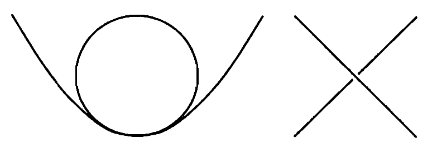
\includegraphics[width = 0.5\textwidth]{../included_media/ex-1-10-eisenbud.png}
\end{center}
The first represents the union of a circle and a parabola in the
  plane and the second shows the union if two skew lines in
  $3$-space. (You may use the Nullstellensatz to prove your answer is right.)
\end{exercise}

\begin{exercise}
  When is $\mathbb{S}^1\subset \field{R}^2$ irreducible?
\end{exercise}


%%% Local Variables:
%%% mode: latex
%%% TeX-master: "main"
%%% End:



\printbibliography

\end{document}

%%% Local Variables:
%%% mode:
%%% TeX-master: t
%%% TeX-engine: xetex
%%% End:
